\section{Học sâu Đo lường (Deep Metric Learning) và Tìm kiếm Ảnh}
\label{sec:deep_metric_learning}

\subsection{Tổng quan: Học cách "Đo lường" Sự tương đồng}
\label{subsec:dml_overview}
Trong các bài toán phân loại, mục tiêu cuối cùng của một mạng nơ-ron là ánh xạ một đầu vào (ảnh) tới một trong $N$ lớp đã được định nghĩa trước. Hàm mất mát Cross-Entropy tối ưu hóa mô hình để đưa ra một dự đoán rời rạc. Tuy nhiên, trong nhiều ứng dụng thực tế, chúng ta không chỉ muốn biết một bức ảnh thuộc lớp nào, mà còn muốn đo lường \textbf{mức độ tương đồng} giữa hai bức ảnh bất kỳ. Ví dụ, hai bức ảnh về hai con chó golden retriever khác nhau nên "gần" nhau hơn nhiều so với một ảnh chó golden retriever và một ảnh mèo.

\textbf{Học sâu Đo lường (Deep Metric Learning - DML)} là một trường phái của học biểu diễn (representation learning) tập trung vào việc học trực tiếp một \textbf{hàm khoảng cách (distance metric)} trong một không gian đặc trưng. Thay vì huấn luyện một bộ phân loại, DML huấn luyện một mạng (thường là CNN hoặc Transformer) để tạo ra các \textbf{vector nhúng (embedding vectors)} sao cho các vector này tuân theo một nguyên lý hình học đơn giản:
\begin{itemize}
	\item Các mẫu \textbf{tương đồng} về mặt ngữ nghĩa (positive pairs) được ánh xạ tới các điểm \textbf{gần nhau} trong không gian nhúng.
	\item Các mẫu \textbf{khác biệt} về mặt ngữ nghĩa (negative pairs) được ánh xạ tới các điểm \textbf{cách xa nhau} trong không gian nhúng.
\end{itemize}

Không gian vector kết quả này được gọi là \textbf{không gian nhúng (embedding space)}, và nó cực kỳ hữu ích cho các ứng dụng như:
\begin{itemize}
	\item \textbf{Tìm kiếm ảnh theo ảnh (Image Retrieval):} Tìm các ảnh tương tự nhất với một ảnh truy vấn.
	\item \textbf{Nhận dạng và Xác minh Khuôn mặt (Face Recognition \& Verification):} Xác định xem hai ảnh khuôn mặt có thuộc về cùng một người hay không.
	\item \textbf{Phân cụm (Clustering):} Tự động gom nhóm các ảnh tương tự mà không cần nhãn.
\end{itemize}

\subsection{Kiến trúc và Các Hàm mất mát Kinh điển}
\label{subsec:dml_architecture_losses}
Một pipeline DML điển hình bao gồm một mạng backbone để trích xuất đặc trưng và một hàm mất mát được thiết kế đặc biệt để cấu trúc hóa không gian nhúng.

\subsubsection{Các Hàm mất mát dựa trên Cặp (Pair-based Losses)}
\label{subsubsec:pair_based_losses}

\paragraph{Contrastive Loss (Siamese Networks):}
Đây là một trong những cách tiếp cận sớm và cơ bản nhất, được phổ biến hóa bởi các mạng \textbf{Siamese Network} \cite{Hadsell2006}.
\begin{itemize}
	\item \textbf{Kiến trúc:} Một mạng Siamese bao gồm hai (hoặc nhiều) nhánh encoder có \textbf{trọng số được chia sẻ (shared weights)}. Hai ảnh đầu vào được đưa qua hai nhánh này để tạo ra hai vector nhúng $\mathbf{z}_1, \mathbf{z}_2$.
	\item \textbf{Mục tiêu:} Hàm mất mát Contrastive Loss được thiết kế để "kéo" các cặp tương đồng lại gần và "đẩy" các cặp khác biệt ra xa một khoảng cách tối thiểu gọi là \textbf{biên (margin)} $m$.
	\begin{equation}
		\mathcal{L}(W, y, \mathbf{x}_1, \mathbf{x}_2) = (1-y) \frac{1}{2} D_W^2 + y \frac{1}{2} \{\max(0, m - D_W)\}^2
	\end{equation}
	Trong đó:
	\begin{itemize}
		\item $D_W = ||f_W(\mathbf{x}_1) - f_W(\mathbf{x}_2)||_2$ là khoảng cách Euclid giữa hai vector nhúng.
		\item $y=0$ nếu cặp $(\mathbf{x}_1, \mathbf{x}_2)$ là tương đồng (positive), và $y=1$ nếu chúng khác biệt (negative).
		\item $m > 0$ là biên. Loss bằng 0 cho một cặp khác biệt nếu khoảng cách giữa chúng đã lớn hơn $m$.
	\end{itemize}
\end{itemize}

\begin{center}
	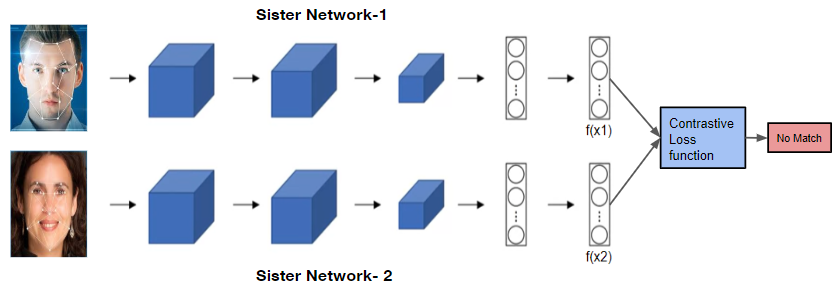
\includegraphics[width=0.8\textwidth]{images/siamese_network_diagram.png}
	\captionof{figure}{Sơ đồ một mạng Siamese. Hai ảnh đầu vào đi qua hai encoder có trọng số chia sẻ để tạo ra các vector nhúng. Hàm mất mát Contrastive Loss sau đó được tính toán dựa trên khoảng cách giữa chúng.}
	\label{fig:siamese_network}
\end{center}
% Keyword gợi ý: siamese network architecture, contrastive loss

\subsubsection{Các Hàm mất mát dựa trên Bộ ba (Triplet-based Losses)}
\label{subsubsec:triplet_based_losses}

\paragraph{Triplet Loss (FaceNet):}
Contrastive Loss chỉ xem xét quan hệ trong từng cặp, nhưng không đảm bảo rằng các lớp khác nhau sẽ được phân tách tốt. \textbf{Triplet Loss}, được giới thiệu trong bài báo \textbf{FaceNet} \cite{Schroff2015} của Google, đã giải quyết vấn đề này bằng cách xem xét mối quan hệ tương đối giữa ba mẫu.
\begin{itemize}
	\item \textbf{Bộ ba (Triplet):} Mỗi mẫu huấn luyện bao gồm ba ảnh:
	\begin{enumerate}
		\item \textbf{Anchor (A):} Một ảnh tham chiếu.
		\item \textbf{Positive (P):} Một ảnh khác cùng lớp với Anchor.
		\item \textbf{Negative (N):} Một ảnh thuộc một lớp khác với Anchor.
	\end{enumerate}
	\item \textbf{Mục tiêu:} Hàm mất mát Triplet Loss yêu cầu khoảng cách từ Anchor đến Positive phải nhỏ hơn khoảng cách từ Anchor đến Negative ít nhất một khoảng biên $m$.
	\begin{equation}
		\mathcal{L}(A, P, N) = \max \left( ||f(A) - f(P)||_2^2 - ||f(A) - f(N)||_2^2 + m, 0 \right)
	\end{equation}
	Loss sẽ bằng 0 nếu điều kiện $||f(A) - f(N)||_2^2 > ||f(A) - f(P)||_2^2 + m$ được thỏa mãn.
\end{itemize}

\begin{center}
	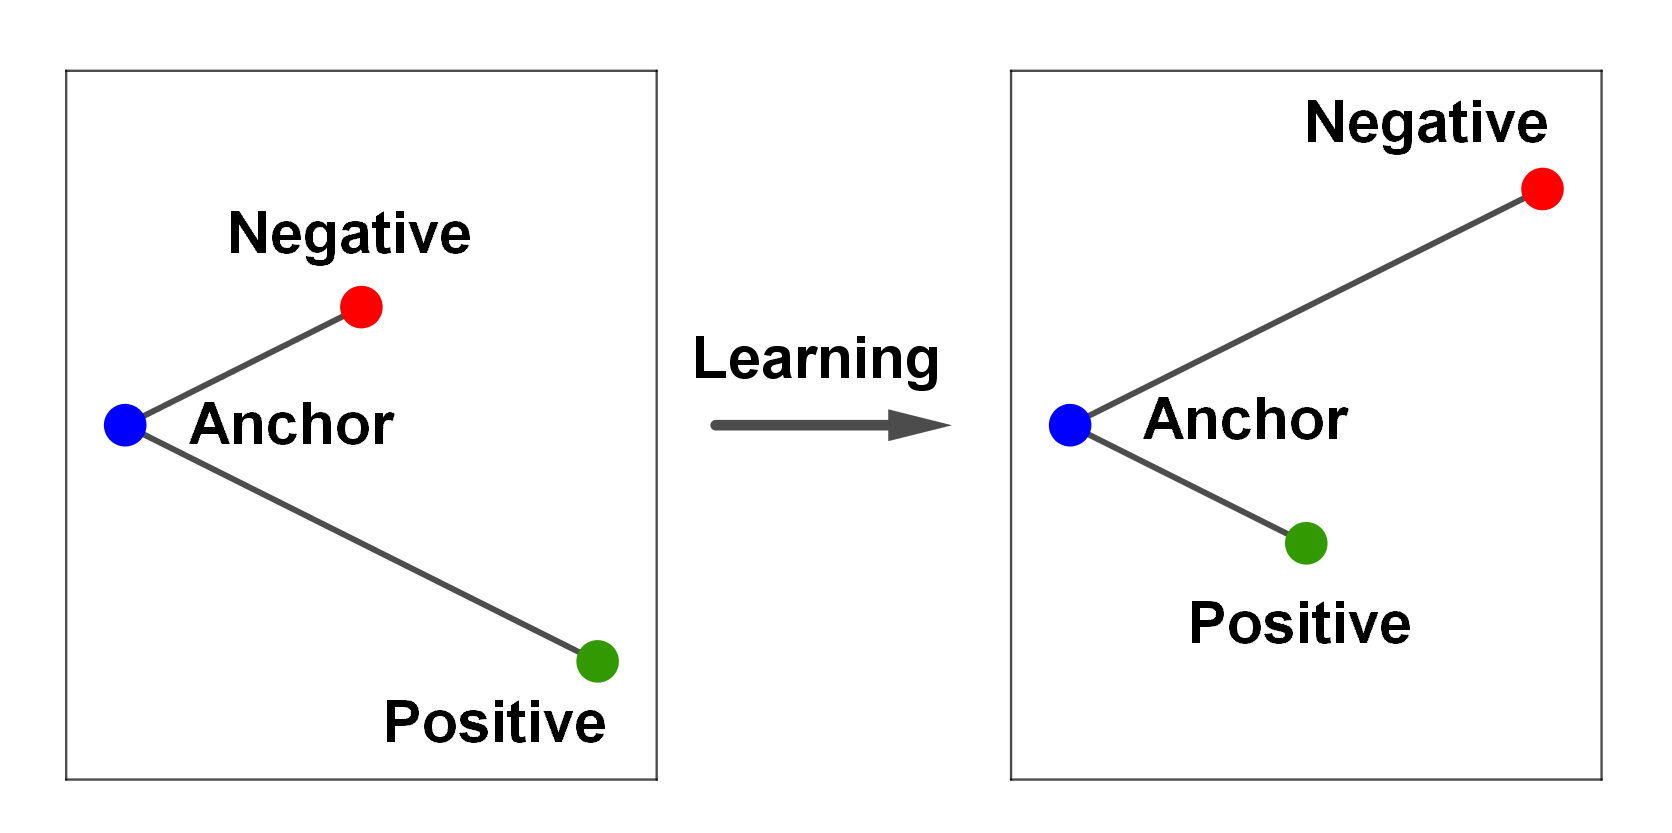
\includegraphics[width=0.9\textwidth]{images/triplet_loss_illustration.png}
	\captionof{figure}{Minh họa nguyên lý của Triplet Loss. Hàm mất mát cố gắng "đẩy" mẫu Negative (N) ra xa khỏi Anchor (A) hơn so với mẫu Positive (P) một khoảng cách ít nhất bằng margin.}
	\label{fig:triplet_loss}
\end{center}
% Keyword gợi ý: triplet loss facenet, deep metric learning triplet

\textbf{Thách thức của Triplet Loss:} Việc chọn các bộ ba "khó" (hard triplets) là rất quan trọng. Nếu chọn các bộ ba quá dễ (ví dụ: N đã ở rất xa A), gradient sẽ bằng 0 và mô hình không học được gì. Các chiến lược \textbf{khai thác bộ ba (triplet mining)} như "hard negative mining" đã được phát triển để tự động tìm các bộ ba hiệu quả nhất trong mỗi mini-batch.

\subsubsection{Các Hàm mất mát Nâng cao và dựa trên Proxy}
\label{subsubsec:advanced_metric_losses}
Để giải quyết các vấn đề về lấy mẫu của Triplet Loss, các hàm mất mát phức tạp hơn đã được đề xuất. Một hướng đi quan trọng là sử dụng các \textbf{"proxy"}.
\begin{itemize}
	\item \textbf{Ý tưởng:} Thay vì so sánh một anchor với các mẫu negative riêng lẻ trong batch, tại sao không so sánh nó với các vector đại diện (proxy) cho mỗi lớp?
	\item \textbf{Proxy-NCA Loss:} Mỗi lớp trong bộ dữ liệu được gán một vector proxy có thể học được. Hàm mất mát sau đó sẽ cố gắng kéo mỗi mẫu lại gần proxy của lớp nó và đẩy nó ra xa các proxy của các lớp khác.
	\item \textbf{Lợi ích:} Phương pháp này giảm độ phức tạp tính toán từ việc so sánh $O(N^2)$ cặp xuống còn $O(N)$ (so sánh với các proxy), giúp huấn luyện hiệu quả hơn trên các bộ dữ liệu lớn với nhiều lớp.
\end{itemize}

\subsubsection{Các Hàm mất mát dựa trên Biên Góc (Angular Margin Losses)}
\label{subsubsec:angular_margin_losses}
Trong các bài toán như nhận dạng khuôn mặt, việc các đặc trưng có độ lớn (magnitude) khác nhau có thể gây nhiễu. Các hàm mất mát dựa trên biên góc được thiết kế để huấn luyện các biểu diễn trên một \textbf{siêu cầu (hypersphere)}, nơi chỉ có góc (đo bằng độ tương đồng cosine) là quan trọng.
\begin{itemize}
	\item \textbf{ArcFace Loss:} \cite{Deng2019} là một trong những phương pháp phổ biến nhất. Nó trực tiếp thêm một \textbf{biên góc (angular margin)} $m$ vào góc $\theta_{y_i}$ giữa embedding của mẫu $x_i$ và trọng số của lớp $y_i$ tương ứng trong lớp phân loại cuối cùng.
	\begin{equation}
		\mathcal{L} = -\frac{1}{N} \sum_{i=1}^{N} \log \frac{e^{s(\cos(\theta_{y_i} + m))}}{e^{s(\cos(\theta_{y_i} + m))} + \sum_{j=1, j\neq y_i}^{C} e^{s\cos\theta_j}}
	\end{equation}
	Bằng cách này, ArcFace buộc các đặc trưng của cùng một lớp phải trở nên "chặt chẽ" hơn trên siêu cầu, tạo ra một không gian nhúng có tính phân biệt cực kỳ cao.
\end{itemize}

\subsection{Ứng dụng: Tìm kiếm Ảnh (Image Retrieval)}
\label{subsec:application_image_retrieval}
Tìm kiếm ảnh dựa trên nội dung (Content-Based Image Retrieval - CBIR) là một trong những ứng dụng tiêu biểu và mạnh mẽ nhất của Deep Metric Learning.

\textbf{Quy trình điển hình:}
\begin{enumerate}
	\item \textbf{Giai đoạn Offline (Indexing):}
	\begin{enumerate}
		\item Huấn luyện một mạng DML (ví dụ: sử dụng Triplet Loss hoặc ArcFace Loss) trên một bộ dữ liệu lớn để học một không gian nhúng hiệu quả.
		\item Đưa toàn bộ các ảnh trong cơ sở dữ liệu (gallery) qua mạng đã huấn luyện để trích xuất các vector nhúng (embedding vectors) cho chúng.
		\item Xây dựng một chỉ mục (index) từ hàng triệu, thậm chí hàng tỷ vector này để hỗ trợ tìm kiếm nhanh.
	\end{enumerate}
	\item \textbf{Giai đoạn Online (Querying):}
	\begin{enumerate}
		\item Khi nhận được một ảnh truy vấn (query image), đưa nó qua cùng một mạng DML để trích xuất vector nhúng.
		\item Sử dụng vector truy vấn này để tìm kiếm các vector gần nhất trong chỉ mục đã xây dựng. Phép đo khoảng cách thường là \textbf{khoảng cách Euclid L2} hoặc \textbf{độ tương đồng Cosine}.
		\item Trả về các ảnh tương ứng với các vector gần nhất được tìm thấy, được xếp hạng theo mức độ tương đồng.
	\end{enumerate}
\end{enumerate}

\begin{mdframed}[style=infobox]
	\textbf{Thách thức của Quy mô: Tìm kiếm Nhanh với ANN}
	
	Việc tìm kiếm tuần tự (brute-force search) trên hàng triệu vector là quá chậm. Do đó, các hệ thống thực tế sử dụng các thuật toán \textbf{Tìm kiếm Lân cận Gần đúng (Approximate Nearest Neighbor - ANN)}.
	\begin{itemize}
		\item \textbf{FAISS (Facebook AI Similarity Search):} Một thư viện mã nguồn mở cực kỳ phổ biến và hiệu quả, cung cấp nhiều thuật toán ANN như Lượng tử hóa Tích (Product Quantization - PQ), HNSW (Hierarchical Navigable Small World graphs), và IVF (Inverted File).
		\item \textbf{ScaNN (Scalable Nearest Neighbors):} Một thuật toán từ Google, cũng rất hiệu quả cho tìm kiếm quy mô lớn.
	\end{itemize}
	Các thuật toán này đánh đổi một chút độ chính xác để đạt được tốc độ tìm kiếm nhanh hơn hàng nghìn lần.
\end{mdframed}

\subsection{Kết nối với các Mô hình Hiện đại}
\label{subsec:dml_modern_connections}
Các nguyên lý của Deep Metric Learning không chỉ tồn tại trong các mô hình chuyên biệt. Chúng chính là nền tảng cho nhiều mô hình nền tảng SOTA hiện nay.
\begin{itemize}
	\item \textbf{CLIP và Học Tương phản Đa phương thức:} Mô hình CLIP của OpenAI \cite{Radford2021} thực chất là một mô hình DML quy mô lớn. Nó sử dụng một hàm mất mát tương phản để học một không gian nhúng chung, nơi vector của một bức ảnh "con chó" sẽ gần với vector của câu văn "bức ảnh một con chó". Điều này cho phép tìm kiếm ảnh bằng văn bản (text-to-image retrieval) một cách hiệu quả.
	\item \textbf{DINOv2 và Học Tự giám sát:} Mô hình DINOv2 của Meta AI \cite{Oquab2023} kết hợp các ý tưởng từ self-supervised learning và DML. Nó học các biểu diễn mạnh mẽ đến mức có thể được sử dụng "ngay lập tức" (off-the-shelf) cho các tác vụ như tìm kiếm ảnh tương tự, phân cụm, và thậm chí là phân đoạn mà không cần fine-tuning.
\end{itemize}
Deep Metric Learning không chỉ là học cách "đo khoảng cách", mà là một bước đi cơ bản để dạy cho máy tính hiểu được "mối quan hệ" giữa các khái niệm thị giác. Nó đã và đang là động lực đằng sau nhiều tiến bộ quan trọng nhất trong thị giác máy tính, từ các ứng dụng thực tế như tìm kiếm sản phẩm đến các mô hình nền tảng có khả năng lý luận đa phương thức.

\section*{Tài liệu tham khảo}
\begin{itemize}
	\item[1] Schroff, F., Kalenichenko, D., \& Philbin, J. (2015). Facenet: A unified embedding for face recognition and clustering. In \textit{Proceedings of the IEEE conference on computer vision and pattern recognition (CVPR)}. (Paper gốc giới thiệu Triplet Loss và FaceNet).
	\item[2] Hadsell, R., Chopra, S., \& LeCun, Y. (2006). Dimensionality reduction by learning an invariant mapping. In \textit{2006 IEEE Computer Society Conference on Computer Vision and Pattern Recognition (CVPR'06)}. (Paper kinh điển giới thiệu Contrastive Loss).
	\item[3] Deng, J., Guo, J., Xue, N., \& Zafeiriou, S. (2019). Arcface: Additive angular margin loss for deep face recognition. In \textit{Proceedings of the IEEE/CVF conference on computer vision and pattern recognition (CVPR)}. (Paper giới thiệu ArcFace Loss).
	\item[4] Radford, A., Kim, J. W., Hallacy, C., Ramesh, A., Goh, G., Agarwal, S., ... \& Sutskever, I. (2021). Learning transferable visual models from natural language supervision. In \textit{International Conference on Machine Learning (ICML)}. (Paper gốc về CLIP).
	\item[5] Oquab, M., Darcet, T., Moutakanni, T., Vo, H., Szafraniec, M., ... \& Joulin, A. (2023). Dinov2: Learning robust visual features without supervision. \textit{arXiv preprint arXiv:2304.07193}. (Paper gốc về DINOv2).
	\item[6] Johnson, J., Douze, M., \& Jégou, H. (2019). Billion-scale similarity search with gpus. \textit{IEEE Transactions on Big Data}, 7(3), 535-547. (Paper giới thiệu thư viện FAISS).
	\item[7] Sohn, K. (2016). Improved deep metric learning with multi-class n-pair loss objective. In \textit{Advances in neural information processing systems (NeurIPS)}. (Giới thiệu N-pair loss).
\end{itemize}